\chapter[Cut locus of a submanifold]{Cut locus of a submanifold}
\minitoc

\hf The cut locus of a point plays an important role in analyzing the local structure of a Riemannian manifold $M$. In the last chapter we had studied cut locus of a point, conjugate locus and some of their properties. Similarly, one can ask about the notion of cut locus for a non-empty subset of $M$. In order to give a similar definition, we need to first define distance minimal geodesics joining a point $p\in M$ to a subset $N\subseteq M$. If $q\in N$ such that the geodesic is distance minimal geodesic joining $p$ and $q$, and it minimizes the distance between the set $N$ and the point $p$ then we call such a geodesic a distance minimal geodesic. Now the cut locus of $N$ consists of all points $q\in M$ such that there exists a distance minimal geodesic which fails to be minimal beyond $q$. Conjugate locus is termed as focal locus if we replace point with submanifold. In this chapter we will study the cut locus of a subset, in particular, a submanifold. We will motivate the results based on some examples and the proofs will be discussed in the subsequent chapters.

\section{Cut locus of submanifolds}\label{sec:cutLocusOfSubmanifolds}
\hfb In order to have a definition of the cut locus for a submanifold (or a subset), we need to generalize the notion of a minimal geodesic.
\begin{defn}\label{distmin}\index{distance minimal geodesic}\index{$N$-geodesic}
    A geodesic $\gamma $ is called a \emph{distance minimal geodesic} joining $N$ to $p$ if there exists $q\in N$ such that $\gamma$ is a minimal geodesic joining $q$ to $p$ and $l(\gamma)= d(p,N) $. We will refer to such geodesics as \textit{$N$-geodesics}.\index{$N$-geodesic}
\end{defn}
\vspace{0.3cm}
\noindent If $N$ is an embedded submanifold, then an $N$-geodesic is necessarily orthogonal to $N$. This follows from the first variational principle. We are ready to define the cut locus for $N\subset M$. 

\begin{defn}[Cut locus of a subset]\index{cut locus of a subset}\label{cutlocus1}
    Let $M$ be a Riemannian manifold and $N$ be any non-empty subset of $M.$ If $\cutn$ denotes the \emph{cut locus of $N$}, then we say that $q\in \cutn $ if and only if there exists a distance minimal geodesic joining $N$ to $q$ such that any extension of it beyond $q$ is not a distance minimal geodesic.
\end{defn}
\bigskip
\begin{eg}\label{eg:Example-cutLocusOfx-Axis}
    Let $M=\mathbb{R}^2$ with the Euclidean metric and $N$ be the $x$-axis. Then the cut locus of $N$ will be empty. If we shoot any geodesic, which are straight lines, perpendicular to $x$-axis, these will never fail to be distance minimal and hence the cut locus will be empty.
    \begin{figure}[!htb]
        \centering
        \incfig[0.5]{Example-CutLocusOfx-Axis}
        \caption{Cut locus of $x$-axis in $\mathbb{R}^2$ }
    \end{figure}
\end{eg}
\vspace{0.3cm}

\begin{eg}\label{eg:Example-cutLocusOfCircle}
    Let $M=\mathbb{R}^{n+1}$ with the Euclidean metric and $N=\mathbb{S}^n$. Then the cut locus will be the center of the sphere. Note that if we shoot a minimal geodesic from any point of $\mathbb{S}^n$, then it fails its minimizing property beyond the origin (see \Cref{fig:Example-CutLocusCircle}). Hence, $\bf{0}$ is a cut point. To see this is the only cut point, we start with any point $\mathbf{a}$ other than origin. Consider a distance minimal geodesic $\gamma$ starting at $\mathbb{S}^n$ to $\mathbf{a}$.  
    \begin{equation*}\label{eq:lineJoiningTwoPoints}
        \gamma(t) = (1-t) \frac{\mathbf{a}}{\left\|\mathbf{a}\right\|}+ t \mathbf{a},~0\le t\le 1.
    \end{equation*}
    Note that 
    \begin{displaymath}
        l(\gamma)=d(P,Q) = \left|1-\left\|\mathbf{a}\right\|\right|.
    \end{displaymath}
    Let $\epsilon=\frac{\left\|\mathbf{a}\right\|}{2}$. Consider the point $R=\gamma(1+\epsilon)$. We have
    \begin{align*}
        l(\gamma)\big|_{[0,1+\epsilon]} = d(P,R).
    \end{align*}
    \begin{figure}[!htbp]
        \centering
        \begin{subfigure}{.45\textwidth}
            \incfig[0.9]{Example-CutLocusCircle}
            \caption{$(0,0)$ is a cut point}
            \label{fig:Example-CutLocusCircle}
        \end{subfigure}
        \begin{subfigure}{.45\textwidth}
            \incfig[0.9]{Example-CutLocusCircle-02}
            \caption{No other points are cut points}
        \end{subfigure}
        \caption{Cut locus of $\mathbb{S}^1$ in $\mathbb{R}^2$}
    \end{figure}
    \noindent Now we will show that $d(\mathbb{S}^n,R)$ is same as the length of $\gamma$. Note that $R=(1+\epsilon)\mathbf{a}-\frac{\epsilon \mathbf{a}}{\left\|\mathbf{a}\right\|}$ which simplifies to $\frac{\mathbf{a}}{2}(1-\left\|\mathbf{a}\right\|) $. Note that 
    \begin{align*}
        d^2(\mathbb{S}^n,R) & = \inf_{\mathbf{x}\in \mathbb{S}^n} d^2 \left(\mathbf{x},\frac{\mathbf{a}}{2}(1-\left\|\mathbf{a}\right\|)\right) 
        \\[1ex]
        & = \min \left\{\left\|\mathbf{x}-{\mathbf{v}}\right\|^2:\|\mathbf{x}\|^2=1\right\},~\mathbf{v}=\frac{\mathbf{a}}{2}(1-\left\|\mathbf{a}\right\|).
    \end{align*}
    Set
    \begin{align*}
        f(\mathbf{x})=\left\|\mathbf{x}-\mathbf{v}\right\|^2,~g(\mathbf{x})= \left\|\mathbf{x}\right\|^2-1.
    \end{align*}
    So we want to minimize $f$ such that $g(\mathbf{x})=0$. 
    \begin{align*}
       \nabla f(\mathbf{x}) - \lambda \nabla g(\mathbf{x})= 0 & \implies (\mathbf{x}-\mathbf{v}) - \lambda \mathbf{x} = 0  \implies \mathbf{x} = \dfrac{\mathbf{v}}{1-\lambda}.
    \end{align*}
    Note that  the above quantity is well defined as $\mathbf{v}\neq 0$. Now we will use the given constrain,
    \begin{align*}
        \left\|\mathbf{x}\right\|=1 & \implies \left\|\mathbf{v}\right\|=|1-\lambda| \\
        & \implies \lambda = 1 \pm \left\|\mathbf{v}\right\| \\
        & \implies \mathbf{x} = \pm \frac{\mathbf{v}}{\left\|\mathbf{v}\right\|} = \pm \frac{\mathbf{a}}{\left\|\mathbf{a}\right\|}.
    \end{align*}
    The point $\frac{\mathbf{a}}{\left\|\mathbf{a}\right\|}$ corresponds to the minima and note that $P=\frac{\mathbf{a}}{\left\|\mathbf{a}\right\|}$. This proves the claim.
\end{eg}

\begin{eg}\label{eg:cutLocusOfS0}
    Let $M=\mathbb{S}^2$ with the round metric and $N=\mathbb{S}^0=\{\mathbf{e}_3,-\mathbf{e}_3\}$, where $\mathbf{e}_3=(0,0,1)$. We claim that the cut locus is the equator, $\{(x,y,0):x^2+y^2=1\}$. Note that if $\gamma$ is an $N$-geodesic (great circle) starting at the North Pole, then it remains distance minimal until it hits the equator circle. As soon as it goes beyond the circle, we can find another geodesic $\eta$ from the South Pole which is shorter and hence $\gamma$ is no longer distance minimal, see \Cref{fig:Example-CutLocus-SphereS0}. 
    \begin{figure}[!htb]
        \centering
        \incfig[0.45]{Example-CutLocus-SphereS0}
        \caption{Cut locus of $\mathbb{S}^0$ in $2$-sphere \label{fig:Example-CutLocus-SphereS0}}
    \end{figure}

    \noindent Therefore, the equator circle is in the cut locus. We also note that any other point not on the equator is either on the top or bottom hemisphere. In either of the cases, a minimal geodesic does not fail its distance minimal property beyond the point. So the cut locus is precisely the circle with $z=0$. By the same argument it follows that the cut locus of $\mathbb{S}^0$ in $\mathbb{S}^n$ is
    \begin{displaymath}
        \mathbb{S}^{n-1}= \left\{(x_0,\cdots,x_{n-1},0): x_0^2+\cdots+x_{n-1}^2=1\right\}.
    \end{displaymath}
\end{eg}

\begin{eg}[Cut locus of equator in $2$-sphere]
    Let $M=\mathbb{S}^2$ with the round metric and $N=\mathbb{S}^1=\{(x,y,0):x^2+y^2=1\}$. The cut locus of $N$ is $\mathbb{S}^0=\left\{\mathbf{e}_3,-\mathbf{e}_3\right\}$. The argument is similar as above.
\end{eg}

% \textcolor{red}{Finding the cut locus of the equator. We claim that the cut locus is the two poles. It is clear that both points are cut points. In order to show that no other points are cut points, take $\mathbf{v} \in \mathbb{S}^2$  such that $\mathbf{v}\notin \mathbb{S}^1$, which is the equator. Note that any distance minimal geodesic, a great circle, must pass through two poles. If we shoot a distance minimal geodesic from $\mathbb{S}^1$ to $\mathbf{v}$, then it must pass through the two poles and hence the circle will be unique. Note that the geodesic $\gamma$ is distance minimal beyond $\mathbf{v}$ as it remains distance minimal till the north pole, see \Cref{fig:Example-CutLocus-SphereS1}.}
%     \begin{figure}[!htpb]
%         \centering
%         \incfig[0.65]{Example-CutLocus-SphereS1}
%         \caption{Cut locus of the equator in $\mathbb{S}^2$ \label{fig:Example-CutLocus-SphereS1}}
%     \end{figure}

\begin{eg}[Join induced by cut locus]\label{join}
    Let $\mathbb{S}_i^k \hookrightarrow \mathbb{S}^n$ denote the embedding of the $k$-sphere in the first $k+1$ coordinates while $\mathbb{S}^{n-k-1}_l$ denote the embedding of the $(n-k-1)$-sphere in the last $n-k$ coordinates. It can be seen that $\textup{Cu}(\mathbb{S}_i^k)=\mathbb{S}_l^{n-k-1}$. In fact, starting at a point $p\in \mathbb{S}^k_i$ and travelling along a unit speed geodesic in a direction normal to $T_p\mathbb{S}^k_i$, we obtain a cut point at a distance $\pi/2$ from $\mathbb{S}^k_i$.
    \begin{figure}[!htpb]
        \centering
        \incfig[0.45]{S2_equator_cutlocus}
        \caption{The cut locus of the equator in $\mathbb{S}^2$\label{fig:S2_equator_cutlocus}}
    \end{figure}
    
    \hf Moreover, in this case $\textup{Cu}(\mathbb{S}_l^{n-k-1})=\mathbb{S}_i^{k}$ and the $n$-sphere $\mathbb{S}^n$ can be expressed as the union of geodesic segments joining $\mathbb{S}_i^k$ to $\mathbb{S}_l^{n-k-1}$. This is a geometric variant of the fact that the $n$-sphere is the (topological) join of $\mathbb{S}^k$ and $\mathbb{S}^{n-k-1}$. We also observe that $\mathbb{S}^n - \mathbb{S}_l^{n-k-1}$ deforms to $\mathbb{S}_i^k$ while $\mathbb{S}^n - \mathbb{S}_i^{k}$ deforms to $\mathbb{S}_l^{n-k-1}$. 
    
    \hf In our example, let $\nu_i^{n-k}$ and $\nu_l^{k+1}$ denote the normal bundles of $\mathbb{S}_i^k$ and $\mathbb{S}_l^{n-k-1}$ respectively. We may express $\mathbb{S}^n$ as the union of normal disk bundles $D(\nu_i)$ and $D(\nu_l)$. These disk bundles are trivial and are glued along their common boundary $\mathbb{S}^k_i\times \mathbb{S}_l^{n-k-1}$ to produce $\mathbb{S}^n$. Moreover, $\mathbb{S}^k_i$ is an analytic submanifold of the real analytic Riemannian manifold $\mathbb{S}^n$ with the round metric. There is a generalization of this phenomenon  \cite[Lemmas 1.3-1.5, Theorem 3.1]{Omo68}.
    \begin{thm}[Omori 1968]
        Let $M$ be a compact, connected, real analytic Riemannian manifold which has an analytic submanifold $N$ such that the cut  point of $N$ with respect to every geodesic, which starts from $N$ and whose initial  direction is orthogonal to $N$ has a constant distance $\pi$ from $N$. Then $N'=\cutn$ is an analytic submanifold and $M$ has a decomposition $M = DN\cup_{\varphi} DN'$, where $DN,  DN'$ are normal disk bundles of $N, N'$ respectively.
    \end{thm}
\end{eg}

\subsection{Separating set}\label{subsec:separatingSet}
\hfb In all the examples in the previous section, we observed the cut locus of any submanifold $N$ is same as the set of all points which has at least two minimal geodesics joining $N$ to the point. This leads to the following definition.

\begin{defn}[Separating set]\label{defn:SeparatingSet}\index{separating set}
    Let $N$ be a subset of a Riemannian manifold $M$. The set $\sen$, called the \textit{separating set}, consists of all points $q\in M$ such that at least two distance minimal geodesics from $N$ to $q$ exist.
\end{defn}
\begin{figure}[!htpb]
    \centering
    \incfig[0.5]{SeparatingSetDescription}
    \caption{Separating set of $N$ \label{fig:SeparatingSet}}
\end{figure}

\vspace{0.3cm}
\hf The following example shows that for a given submanifold $N\subseteq M$, the separating set need not be same as the cut locus.

\begin{eg}[Cut locus of ellipse]\label{eg:CutLocusOfEllipse}
    Let $M=\mathbb{R}^2$ with the Euclidean metric and $N= \left\{(x,y):\frac{x^2}{a^2}+\frac{y^2}{b^2}=1\right\}$ for some non-zero real numbers $a$ and $b$ with $a\neq b$.
    \begin{figure}[!htb]
        \centering
        \incfig[0.5]{Example-CutLocusEllipse}
        \caption{$\cutn$ and $\sen$ \label{fig:Example-CutLocusEllipse}}
    \end{figure}
    Let $A=(-a,0)$ and $B=(a,0)$ be two foci of the ellipse. Note that for any point $C=(x,0)$ with $x\in (-a,a)$, we have two $N$-geodesics joining $N$ to $C$. Hence, all the points are separating point (see \Cref{fig:Example-CutLocusEllipse}). However, the two foci are not separating points, but they are in the cut locus. So $\sen \neq \cutn$. 
\end{eg}

\vspace{0.3cm}
\noindent Note that $\sen\subset \cutn$. Although the sets $\sen$ and $\cutn$ are not same, in general, we can ask whether including the limit points of $\sen$ make them equal. In the next chapter, we will see that indeed this is the case, and we have $\overline{\sen}=\cutn$ (\Cref{thm:SeClosureIsCutLocus}). \label{Page:SeClosureIsCu} This, in particular, proves that cut locus is a closed set. In general, the cut locus of a subset need not be closed, as illustrated by the following example \cite{TaSa16}.
\begin{eg}[Sabau-Tanaka 2016]
    Consider $\rbb^2$ with the Euclidean inner product. Let $\curlybracket{\theta_n}$, with $\theta_1\in (0,\pi)$, be a decreasing sequence converging to $0$. Let $\overline{B(\mathbf{0},1)}$ be the closed unit ball centered at $(0,0)$. Suppose $B_n:=B(q_n,1)$ is the open ball with radius $1$ and centered at $q_n$. We have chosen $q_n$ such that it does not belong to $\overline{B(\mathbf{0},1)}$ and denotes the center of the circle passing through $p_n=(\cos\theta_n,\sin\theta_n)$ and $p_{n+1} = (\cos\theta_{n+1},\sin\theta_{n+1})$. Define $ N\subset \rbb^2$ by
    \begin{displaymath}
        N \defeq \overline{B(\mathbf{0},1)}\setminus \cup_{n=1}^\infty B(q_n,1).
    \end{displaymath}
    \begin{figure}[!htpb]
        \centering
        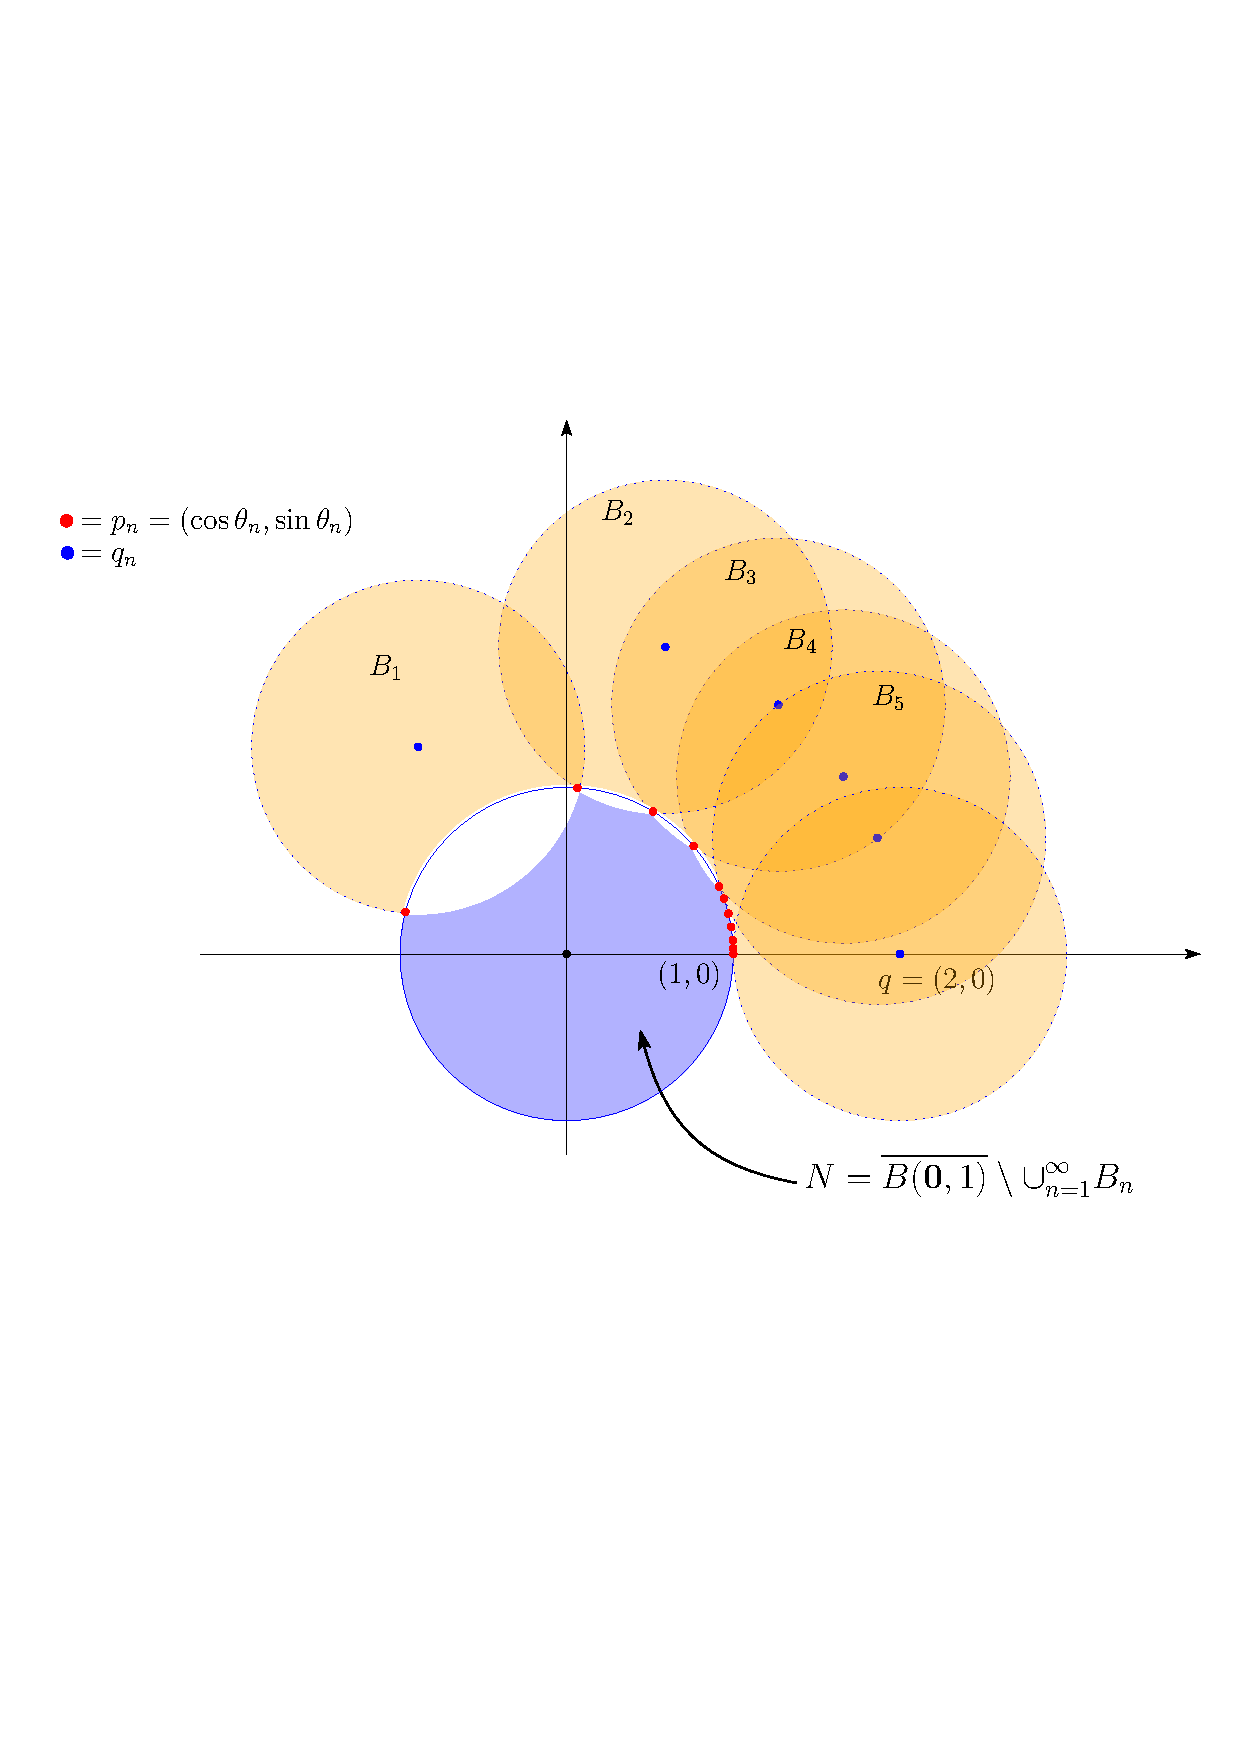
\includegraphics[scale=0.7]{CutLocus-ceg.pdf}
        \caption{Cut locus need not be closed}
        \label{fig:CutLocusNotClosed}
    \end{figure}
    
    \noindent Note that $N$ is a closed set and the sequence $\curlybracket{q_n}$ of cut points of $N$ converges to the point $(2,0)$. However, $(2,0)$ is not a cut point of $N$.
\end{eg}

\hf Using the characterization of cut locus in terms of the separating set, we will list some more examples. Most of the justification is provided by the help of pictures. 

\begin{eg}[Cut locus of $k$ points on the unit circle]
    Let $M=\mathbb{S}^1$ with the round metric and $N=\{A_1,A_2,A_3\}$. Then the cut locus will be $\{B_{12},B_{23},B_{31}\}$, see \Cref{fig:Example-CutLocus-CircleThreePoints}.
    \begin{figure}[!htpb]
        \centering
        \incfig[0.45]{Example-CutLocus-CircleThreePoints}
        \caption{Cut locus of three points on unit circle \label{fig:Example-CutLocus-CircleThreePoints}}
    \end{figure}
    The above example can be generalized for any $k$-points on $\mathbb{S}^1$. The cut locus of $\{A_1,A_2,\cdots,A_k\}$ will be $\{B_{12},B_{23},\cdots, B_{k1}\}$ where $B_{i i+1}$ is the mid-point of $A_i$  and $A_{i+1}$.
\end{eg}

\begin{eg}[Cut locus of $k$ points on $\mathbb{S}^2$]\label{eg:cutLocusOfkPoints}
    Let $A_1,A_2$ and $A_3$ be three points on the equator. The cut locus will be half great circles passing through the mid-points $B_{12},B_{23}$ and $B_{31}$, see \Cref{fig:Example-CutLocus-SphereThreePoints}. In fact, all these semicircles are the separating set of $\{A_1,A_2,A_3\}$, being closed the closure is itself. So, the cut locus is homotopic to wedge of two circles. 
    \begin{figure}[!htpb]
        \centering
        \begin{subfigure}{0.65\textwidth}
            \centering
            \incfig[0.55]{Example-CutLocus-SphereThreePoints}
            \caption{Cut locus of three points in $\mathbb{S}^2$}
            \label{fig:Example-CutLocus-SphereThreePoints}
        \end{subfigure}
        \begin{subfigure}{0.25\textwidth}
            \centering
            \incfig[0.8]{Example-CutLocus-SphereThreePoints-02}
            \caption{Cut locus is homotopic equivalent to $\mathbb{S}^1\vee \mathbb{S}^1$ }
            \label{fig:Example-CutLocus-SphereThreePoints-02}
        \end{subfigure}
        \caption{Cut locus of three points in $\mathbb{S}^2$}
    \end{figure}
    The same can be generalized for $k$-points on the equator of $\mathbb{S}^2$ to conclude that the cut locus is homotopic to $\vee_{k-1}\mathbb{S}^1$.  Similarly, one can show that cut locus of $k$-points in $\mathbb{S}^n$ is homotopic to $\vee_{k-1}\mathbb{S}^{n-1}$. In this example also, the separating set is same as the cut locus as the separating set is closed. 
\end{eg}

\hf The above example, in particular, shows that cut locus need not be a manifold.

\begin{eg}
    Let $M=\mathbb{R}^2$ with the Euclidean metric and $N$ be the wedge of two circles. The cut locus of $N$ consists of centers of these two circles and the $y$-axis with origin removed, see \Cref{fig:Example-CutLocus-Figure8}.
    \begin{figure}[!htb]
        \centering
        \incfig[0.6]{Example-CutLocus-Figure8}
        \caption{Cut locus of wedge of two circles in $\mathbb{R}^2$}
        \label{fig:Example-CutLocus-Figure8}
    \end{figure}
    In fact, if we take any other point then that is not a cut point as any geodesic, a straight line, never fails its distance minimal property. This example, also shows that the cut locus of a subset need not be a closed set.
\end{eg}

\begin{eg}
    Let $M$ be the cylinder $\mathbb{S}^1\times \mathbb{R}$ with the product metric. Let $N=\{\mathbf{v}\}\times \mathbb{R}$ for some $\mathbf{v} \in \mathbb{S}^1$. Then cut locus of $N$ is $\{-\mathbf{v}\}\times \mathbb{R}$, see \Cref{fig:Example-CutLocus-Cylinder-Submanifold}. 
    \begin{figure}[!htpb]
        \centering
        \incfig[0.35]{Example-CutLocus-Cylinder-Submanifold}
        \caption{Cut locus of a line on cylinder \label{fig:Example-CutLocus-Cylinder-Submanifold}}
    \end{figure}
    
\end{eg}

\section{An illuminating example}\label{Sec:IlluminatingExample}
\hfb Let $ M = M(n,\rbb) $ be the set of $n\times n$ matrices, and $ N=O(n,\rbb) $ be the set of all orthogonal $n\times n$ matrices. Let $A,B\in M(n,\rbb)$. We fix the standard flat Euclidean metric on $M(n,\rbb)$ by identifying it with $\mathbb{R}^{n^2}$. This induces a distance function given by
\begin{equation*}\label{Example 1 Eq: 1}
	d(A,B) \defeq \sqrt{\trace{(A-B)^T(A-B)}}
\end{equation*}
Consider the distance squared function
\begin{displaymath}
    f: GL(n,\rbb)\to \rbb,~~ A\mapsto d^2(A, O(n,\rbb)).
\end{displaymath}
In order to study this function, we want a closed formula for it.
\begin{lemma}
    The function $f$ can be explicitly expressed as 
    \begin{equation}\label{eq:d2On}
        f(A) = n + \trace{A^TA} - 2\trace{\sqrt{A^TA}}.
    \end{equation} 
\end{lemma}

\begin{proof}
 Let $A\in GL(n,\rbb)$ be any invertible matrix. Then,
\begin{align}
    f(A) & =  \inf_{B\in O(n,\rbb)}d^2(A,B)\nonumber
    \\
         & =  \inf_{B\in O(n,\rbb)} \|A-B\|^2\nonumber
         \\
         & =  \inf_{B\in O(n,\rbb)} \trace{(A-B)^T(A-B)}\nonumber
         \\
         & =  \inf_{B\in O(n,\rbb)} \trace{A^TA-A^TB-B^TA+B^TB}\nonumber
         \\
         & =  \inf_{B\in O(n,\rbb)} \big[\trace{A^TA}-\trace{A^TB}-\trace{B^TA}+\trace{B^TB} \big]\nonumber
         \\
         & =  \trace{A^TA} + \inf_{B\in O(n,\rbb)}\big[- 2\trace{A^TB} \big] + n \nonumber
         \\
         & =  \trace{A^TA} -2\sup_{B\in O(n,\rbb)} \trace{A^TB} + n.  \label{maxdist}
\end{align}
The problem of computing $f(A)$ is equivalent to maximizing the function
\begin{displaymath}
    h_A: O(n,\rbb)\to \rbb, B\mapsto \trace{A^TB}.
\end{displaymath} 
\paragraph{\blue{Case I:}} $A$ is a diagonal matrix with positive entries. Then, 
\begin{align*}
    \left|h_A(B)\right|  = \left|\trace{A^TB}\right|
     = \left|\sum_{i=1}^n a_{ii} b_{ii} \right| 
     \le \sum_{i=1}^n \abs{a_{ii}b_{ii}}
      & \le \sum_{i=1}^n a_{ii}
    = \trace{A^T} 
    = h_A(I).
\end{align*}
Thus, one of the maximizer is $B=I.$
\paragraph{\blue{Case II:}}  For any non-singular matrix $A$, we will use the \textit{singular value decomposition} (SVD). \index{singular value decomposition} Write $A=UDV^T$, where $U$ and $V$ are $n\times n$ orthogonal matrices and $D$ is a diagonal matrix with positive entries. For any $B\in O(n,\rbb)$ using the cyclic property of the trace we have
\begin{align}
    \trace{A^TB}  & = \trace{VDU^TB} = \trace{D(U^TBV)}.
\end{align}
Since $U^TBV$ is an orthogonal matrix, maximizing over $B$ reduces to the earlier observation that $B$ will be a maximizer if $U^TBV = I$, which implies $B = UV^T$. 

\vspace{0.3cm}
\hf Since $A$ is invertible, by the polar decomposition, there exists an orthogonal matrix $Q$ and a symmetric positive definite matrix $S=\sqrt{A^TA}$ such that $A=QS$. As $S$ is symmetric matrix we can diagonalize it, that is, $S = P\tilde{D}P^T$, where $P\in O(n,\rbb)$ and $\tilde{D}$ is a diagonal matrix. Thus,
\begin{displaymath}
    A = QS = Q P\tilde{D}P^T.
\end{displaymath}
Set $U=QP$, $V=P$ to obtain the SVD of $A$. In particular, the minimizer is given by
$$B=Q=A\big(\sqrt{A^TA}\big)^{-1}.$$
Therefore, 
	\begin{equation*}
		f(A) = n+\trace{A^TA}  - 2\,\trace{\sqrt{A^TA}}
	\end{equation*}
for invertible matrices. 

\vspace{0.3cm}
\hf To find out $f(A)$ for a non-invertible matrix $A$, we note that $GL(n,\rbb)$ is dense in $M(n,\rbb)$ and that $\sqrt{A^TA}$ is well-defined for $A\in M(n,\rbb)$. The continuity of the map $A\mapsto \sqrt{A^T A}$ on $M(n,\rbb)$ implies that the same formula \eqref{eq:d2On} for $f$ applies to $A$ as well. 
\end{proof}

\noindent In order to understand the differentiability of $f$, it suffices to analyze the function $A\mapsto \trace{\sqrt{A^TA}}$. 
\begin{lemma}
	The map $g : M(n,\rbb)\to \rbb, ~A\mapsto \trace{\sqrt{A^TA}}$ is differentiable if and only if $A$ is invertible. 
\end{lemma}

\begin{proof}
    Let $A$ be an invertible matrix. We will prove that the function $g$ is differentiable at $A$. Let $\cali{P}$  be the set of all positive definite matrices which is an open subset of the set of all symmetric matrices $\cali{S}$. We will prove that the map 
    \begin{displaymath}
        r : \cali{P}\to \cali{P}, ~ A\mapsto \sqrt{A}
    \end{displaymath}
    is differentiable. Define a function 
    \begin{displaymath}
        s : \cali{P}\to \cali{P},~ A\mapsto A^2.
    \end{displaymath}
    We will show that $s$ is a diffeomorphism and from the inverse function theorem $r$ will be differentiable. In order to show that $s$ is a diffeomorphism, we claim that for $A\in \cali{P},~ds_{A}:T_{A}\cali{P}\to T_{A^2}\cali{P}$ is injective. Note that $\cali{P}$ is an open subset of a vector space $\cali{S}$ and therefore, $T_{A}\cali{P}\isom \cali{S} \isom T_{A^2}\cali{P}.$ So, take $B\in \cali{S}$ such that $ds_{A}(B) = 0$. We will show that $B = 0.$ Recall that $ds_{A}(B) = AB +BA.$ Now choose an orthonormal basis $\{\vbf_1,\vbf_2,\cdots,\vbf_n\}$ of eigenspace of $A$ and $A\vbf_{i} = \lambda_{i} \vbf_i$ ($\lambda_i>0$). Then,
    \begin{displaymath}
        A(B\vbf_i) = -BA\vbf_i = -B\lambda_i\vbf_i = -\lambda i(B\vbf_i)
    \end{displaymath} 
    which implies $Bv_{i}$ is also an eigenvector of $A$ with eigenvalue $-\lambda_{i}<0$. Hence, $Bv_{i} = 0$ which implies $B=0$.\\
    \hspace{0.7cm} For the converse, we will show that if $A$ is a singular matrix, then the map $g$ is not directional differentiable. Let $A$ be a singular matrix. Using the singular value decomposition, we write 
    \begin{displaymath}
        A = U \begin{pmatrix}
            D & 0 \\ 
            0   & 0_k
        \end{pmatrix} V^T,    
    \end{displaymath}
    where $D$ is a $(n-k)\times (n-k)$ diagonal matrix with positive entries. If 
    \begin{displaymath}
        B = U \begin{pmatrix}
            0_{n-k} & 0 \\
            0 & I_k
        \end{pmatrix}    
    \end{displaymath}
    then we claim that $g$ is not differentiable in the direction of $B$. Since 
    \begin{displaymath}
        \sqrt{(A+tB)^T(A+tB)} = V \begin{pmatrix}
            D & 0 \\
            0 & I_k|t|
        \end{pmatrix} V^T
    \end{displaymath}
    the limit 
    \begin{align*}
        \lim_{t\to 0} \dfrac{g(A+tB) - g(A)}{t} & = \lim_{t\to 0} \dfrac{\trace{V\begin{pmatrix}
            D & 0 \\
            0 & I_k|t|
        \end{pmatrix} V^T} - \trace{V \begin{pmatrix}
            D & 0 \\
            0 & 0_k
        \end{pmatrix} V^T}}{t}\\
        & = k \lim_{t\to 0} \dfrac{|t|}{t} 
    \end{align*}
    does not exist and hence the function $g$ is not differentiable.
\end{proof}

\begin{prop}\label{prop:derivativeOfSqrtMatrixMap}
    If $A$ is an invertible matrix, then 
    \begin{equation}\label{derivativeOfSquareRoot}
        dg_A(H) = \innerprod{A\paran{\sqrt{A^TA}}^{-1}}{H},
    \end{equation}
    where $H$ is a symmetric matrix of order $n$.
\end{prop}

\vspace{0.3cm}
\noindent The following lemma along with chain rule will prove the above proposition. 
\begin{lemma} \label{lem:derivativeOfSquareRoot}
    Let $A$ be a positive definite matrix and $\psi:A\mapsto \sqrt{A}$. Then 
    \begin{equation*}\label{eq: sqrtderivative}
        d\psi_A(H) = \int_0^\infty e^{-t\sqrt{A}}He^{-t\sqrt{A}}~dt,
    \end{equation*}
    for any symmetric matrix $H.$
\end{lemma}

\begin{proof}
    As $\psi(A)\cdot \psi(A) = A$, differentiating at $A$ we obtain
    \begin{equation}\label{eq: sylvester}
            d\psi_A(H)\psi(A) + \psi(A)d\psi_A(H) = H.
    \end{equation}
    We will show the following:
    \begin{enumerate}
        \item [(i)] For any positive definite matrix $X$ and for any symmetric matrix $Y$ the integral 
        \begin{equation}\label{eq: matsqrtderivative}
            \int_0^\infty e^{-tX}Ye^{-tX}~\mathrm{d}t
        \end{equation}
        converges. We note that the eigenvalues of $e^{-tX}$ are $e^{-t\lambda_j}$, where $\lambda_j$ are the eigenvalues of $X$. Since $X$ is a positive definite matrix, each of the $\lambda_j$ is positive. Without loss of generality, we assume that $\lambda=\lambda_1$ is the smallest eigenvalue of $X$. Then we have
        \begin{align*}
            e^{-t \lambda_j} \le e^{-t \lambda} & \implies \left\|e^{-tX}\right\| = e^{-t \lambda}.
        \end{align*} 
        where  $\|\cdot\|$ is the operator norm.  Therefore, the operator norm of the integrand in \eqref{eq: matsqrtderivative} is bounded by $2e^{-t \lambda}\|Y\|$, which is an integrable function. Hence, the integral given by \eqref{eq: matsqrtderivative} converges. 
    
        \item [(ii)] The matrix $d\psi_A(H)$ satisfies \eqref{eq: sylvester}. Observe that 
        \begin{align*}
                & \paran{\int_0^\infty e^{-t\sqrt{A}}\cdot H\cdot e^{-t\sqrt{A}} \mathrm{d}t } \sqrt{A} + \sqrt{A} \paran{\int_0^\infty e^{-t\sqrt{A}}\cdot H\cdot e^{-t\sqrt{A}}~\mathrm{d}t} 
            \\
            = & \int_0^\infty\paran{e^{-t\sqrt{A}}\cdot H\cdot e^{-t\sqrt{A}}  \sqrt{A} + \sqrt{A} e^{-t\sqrt{A}}\cdot H\cdot e^{-t\sqrt{A}}}~\mathrm{d}t
            \\
            = & \int_0^\infty-\paran{e^{-t\sqrt{A}} H e^{-t\sqrt{A}}}'~\mathrm{d}t = H.
        \end{align*}
    \end{enumerate}
    From (i), (ii) and the uniqueness of the derivative, the lemma is proved. 
\end{proof}

\vspace{0.3cm}
\noindent We now give a proof of \Cref{prop:derivativeOfSqrtMatrixMap}.
\begin{proof}[Proof of \Cref{prop:derivativeOfSqrtMatrixMap}]
    Note that using \Cref{lem:derivativeOfSquareRoot}, for any symmetric matrix $H$ we have
    \begin{equation}\label{eq:derivativeOfSquareRoot}
        dg_A(H) = \trace{\int_0^\infty e^{-t\sqrt{A^TA}}\paran{A^TH+H^TA}e^{-t\sqrt{A^TA}}~dt}.
    \end{equation}
    Let us simplify the above expression to get the desired result.
    \begin{align*}
        dg_A(H) & = \int_0^\infty \squarebracket{\trace{e^{-2t\sqrt{A^TA}}H^TA} + \trace{e^{-2t\sqrt{A^TA}}A^TH}}~dt
        \\[1ex] 
        & = \trace{\int_0^\infty e^{-2t \sqrt{A^TA}}H^TA~dt} + \trace{\int_0^\infty e^{-2t \sqrt{A^TA}}A^TH~dt}
        \\[1ex]
        & = \trace{\squarebracket{\int_0^\infty e^{-2t \sqrt{A^TA}}~dt}H^TA} + \trace{\squarebracket{\int_0^\infty e^{-2t \sqrt{A^TA}}~dt}A^TH}
        \\[1ex]
        \begin{split}
            & = \trace{\squarebracket{-\dfrac{\paran{\sqrt{A^TA}}^{-1}}{2} \int_0^\infty \dfrac{d}{dt}e^{-2t\sqrt{A^TA}}~dt}H^TA} 
            \\[0.5ex]
            & \kern 1cm + \trace{\squarebracket{-\dfrac{\paran{\sqrt{A^TA}}^{-1}}{2} \int_0^\infty \dfrac{d}{dt}e^{-2t\sqrt{A^TA}}~dt}A^TH}
        \end{split}
        \\[1ex]
        & = \trace{\dfrac{\paran{\sqrt{A^TA}}^{-1}}{2}H^TA}  + \trace{\dfrac{\paran{\sqrt{A^TA}}^{-1}}{2}A^TH}
        \\[1ex]
        & =  \dfrac{1}{2} \trace{\paran{\sqrt{A^TA}}^{-1}A^TH} + \dfrac{1}{2}  \trace{A^TH\paran{\sqrt{A^TA}}^{-1}}
        \\
        & =  \trace{\paran{\sqrt{A^TA}}^{-1}A^TH}
         = \innerprod{A\paran{\sqrt{A^TA}}^{-1}}{H}
    \end{align*}
    Thus, 
    \begin{equation*} \label{differentialOfSquareRootFinal}
	    dg_A(H) = \innerprod{A\paran{\sqrt{A^TA}}^{-1}}{H}.
    \end{equation*}
\end{proof}
\vspace{0.3cm}
\hspace*{0.5cm}For  any $A\in GL(n,\rbb)$
\begin{equation*}\label{gradfForGL}
    df_A  = 2A-2A\paran{\sqrt{A^TA}}^{-1}=-2A \paran{\sqrt{A^TA}^{-1}-I}.
\end{equation*}
Hence, the negative gradient of the function $f$, restricted to $GL(n,\rbb)$ is given by 
\begin{displaymath}
	-\grad f\big|_A = 2A\paran{\sqrt{A^TA}^{-1}-I}.
\end{displaymath}
The critical points are orthogonal matrices. If $\gamma(t)$ is an integral curve of $-\grad f$ initialized at $A$, then $\gamma(0)=A$ and 
\begin{equation}
\dfrac{d\gamma}{dt} =-2\gamma(t)+2\gamma(t)\paran{\sqrt{\gamma(t)^T\gamma(t)}}^{-1}=-2\gamma(t)+2\paran{\gamma(t)^T}^{-1}\sqrt{\gamma(t)^T\gamma(t)} \label{eq: 4.5}.
\end{equation}
Take the test solution of \eqref{eq: 4.5} given by
\begin{equation}\label{eq: 4.6}
\gamma(t)  = Ae^{-2t} + (1-e^{-2t})\paran{A^T}^{-1}\sqrt{A^TA} = Ae^{-2t} + (1-e^{-2t})A\paran{\sqrt{A^TA}}^{-1}.
\end{equation}
% Observe that, 
% \begin{align*}
% 	Df_A & = 2A - 2A \paran{\sqrt{A^TA}^{-1}}\\
% 		 & = 2A - 2\paran{A^T}^{-1}\sqrt{A^TA}.
% \end{align*}
% And, hence 
% \begin{align}
% 	\dfrac{d\gamma(t)}{dt} = -2\gamma(t)+ 2\paran{\gamma(t)^T}^{-1}\sqrt{\gamma(t)^T\gamma(t)}.\label{eq:4.7}
% \end{align}
\noindent In order to show that $\gamma(t)$ satisfies \eqref{eq: 4.5}, note that
\begin{align*}
    \begin{split}
		\gamma(t)^T\gamma(t) & = \squarebracket{Ae^{-2t}+(1-e^{-2t})\paran{A^T}^{-1}\sqrt{A^TA}}^T\\
        & \qquad \qquad \squarebracket{Ae^{-2t}+(1-e^{-2t})\paran{A^T}^{-1}\sqrt{A^TA}}  
    \end{split}
    \\[1ex]
    \begin{split}
        & = \squarebracket{A^Te^{-2t} +(1-e^{-2t})\sqrt{A^TA} A^{-1}} \\
        & \qquad \qquad \squarebracket{Ae^{-2t}+(1-e^{-2t})\paran{A^T}^{-1}\sqrt{A^TA}}
    \end{split}
    \\[1ex]
    \begin{split}
        & = A^TAe^{-4t} + 2e^{-2t}(1-e^{-2t})\sqrt{A^TA}\\
        & \qquad \qquad +(1-e^{-2t})^2\paran{\sqrt{A^TA} A^{-1} \aTransInverse \sqrt{A^TA}}
    \end{split}
    \\[1ex] 
    \begin{split}
        & = A^TAe^{-4t} + 2e^{-2t}(1-e^{-2t})\sqrt{A^TA}\\
        & \qquad \qquad +(1-e^{-2t})^2\paran{\sqrt{A^TA} \paran{A^TA}^{-1} \sqrt{A^TA}}
    \end{split}
    \\[1ex]
    \begin{split}
        & = A^TAe^{-4t} + 2e^{-2t}(1-e^{-2t})\sqrt{A^TA}\\
        & \qquad \qquad +(1-e^{-2t})^2\paran{\sqrt{A^TA} \sqrtATransAInverse \sqrtATransAInverse \sqrt{A^TA}}
    \end{split}
    \\[1ex] 
    & = A^TAe^{-4t} + 2e^{-2t}(1-e^{-2t})\sqrt{A^TA} + \paran{1-e^{-2t}}^2I\\
    & = \paran{\sqrt{A^TA}~e^{-2t}+\paran{1-e^{-2t}}I}^2.
\end{align*}
Thus,
\begin{displaymath}
    \gamma(t)^T\gamma(t) = \paran{\sqrt{A^TA}~e^{-2t}+\paran{1-e^{-2t}}I}^2
\end{displaymath}
and hence
\begin{displaymath}
    \paran{\sqrt{\gamma(t)^T\gamma(t)}}^T = \paran{\sqrt{A^TA}A^{-1}\gamma(t)}^T = \gamma(t)^T\aTransInverse \sqrt{A^TA}
\end{displaymath}

\noindent This implies that 
\begin{align*}
    \sqrt{\gamma(t)^T\gamma(t)} & = \sqrt{A^TA}\paran{e^{-2t}I+\sqrtATransAInverse \paran{1-e^{-2t}}}\nonumber\\
    \implies \sqrt{\gamma(t)^t\gamma(t)} & = \sqrt{A^TA}A^{-1}\gamma(t)\nonumber\\
    \implies \paran{\sqrt{\gamma(t)^T\gamma(t)}}^T & = \paran{\sqrt{A^TA}A^{-1}\gamma(t)}^T = \gamma(t)^T\aTransInverse \sqrt{A^TA}\nonumber\\
    \implies \paran{\gamma(t)^T}^{-1} \sqrt{\gamma(t)^T\gamma} & = \aTransInverse\sqrt{A^TA}.
\end{align*}
\noindent The right hand side of \eqref{eq: 4.5}, with the test solution, can be simplified to 
\begin{displaymath}
-2Ae^{-2t} + 2e^{-2t}\aTransInverse \sqrt{A^TA}
\end{displaymath}
which is the derivative of $\gamma$. Thus, $\gamma(t)$, as defined in \eqref{eq: 4.6}, is the required flow line which deforms $GL(n,\rbb)$ to $O(n,\rbb).$ In particular, $GL^+(n,\rbb)$ deforms to $SO(n,\rbb)$ and other component of $GL(n,\rbb)$ deforms to $O(n,\rbb)\setminus SO(n,\rbb)$. We note, however, that this deformation takes infinite time to perform the retraction.
\begin{rem}
A modified curve
\begin{equation}\label{GLdefOver1}
\eta(t)=A(1-t)+tA\paran{\sqrt{A^TA}}^{-1}
\end{equation}
with the same image as $\gamma$, defines an actual deformation retraction of $GL(n,\rbb)$ to $O(n,\rbb)$. Apart from its origin via the distance function, this is a geometric deformation in the following sense. Given $A\in GL(n,\rbb)$, consider its columns as an ordered basis. This deformation deforms the ordered basis according to the length of the basis vectors and mutual angles between pairs of basis vectors in a geometrically uniform manner. This is in sharp contrast with Gram-Schmidt orthogonalization, also a deformation of $GL(n,\rbb)$ to $O(n,\rbb)$, which is asymmetric as it never changes the direction of the first column, the modified second column only depends on the first two columns and so on.
\end{rem}
\hspace*{0.5cm}We now show that $f$ is Morse-Bott.\index{Morse-Bott functions} The tangent space $T_I O(n,\rbb)$ consists of skew-symmetric matrices while the normal vectors at $I_n$ are the symmetric matrices. As left translation by an orthogonal matrix is an isometry of $M(n,\rbb)$, normal vectors at $A\in O(n,\rbb)$ are of the form $AW$ for symmetric matrices $W$. Since 
\begin{displaymath}
	df_A(H) = 2\innerprod{A}{H}-2\innerprod{A\big(\sqrt{A^TA}\big)^{-1}}{H}
\end{displaymath}
the relevant Hessian is 
\begin{equation*}
	\hess(f)_A(H,H') = \lim_{t\to 0}\dfrac{df_{A+tH'}(H)-df_A(H)}{t} 
\end{equation*}
with $H=AW, H'=AW'$ and symmetric matrices $W,W'$. Solving the Hessian expression, we have
\begin{align*}
	\hess(f)_A(H,H') 
		& = \lim_{t\to 0} \left(\dfrac{2\innerprod{A+tH'}{H} - 2\innerprod{(A+tH')\sqrt{(A+tH')(A+tH')^T}^{-1}}{H}}{t}\right.
		\\
		& \qquad \qquad \qquad \left. -\dfrac{2\innerprod{A}{H}-2\innerprod{A\sqrt{A^TA}^{-1}}{H}}{t} \right)
	\\[1ex]
	\begin{split}
		& = \lim_{t\to 0} \left( \dfrac{2\innerprod{A}{H}+2t\innerprod{H'}{H}-2\innerprod{A\sqrt{(A+tH')^T(A+tH')}^{-1}}{H}}{t} \right. 
		\\
		& \kern -.5cm \left. -\dfrac{2t\innerprod{H'\sqrt{(A+tH')^T(A+tH')}^{-1}}{H} + 2\innerprod{A}{H}-2\innerprod{A\sqrt{A^TA}^{-1}}{H}}{t} \right)
	\end{split}
	\\[1ex]
	\begin{split}
		& = \lim_{t\to 0} \left( \dfrac{2t\innerprod{H'}{H}-2t\innerprod{H'\sqrt{(A+tH')^T(A+tH')}^{-1}}{H}}{t} \right. 
		\\ 
		& \qquad \qquad \left. \dfrac{-2\innerprod{A\sqrt{(A+tH')^T(A+tH')}^{-1}}{H}+2\innerprod{A\sqrt{A^TA}^{-1}}{H}}{t} \right)
	\end{split}
	\\[1ex]
	\begin{split}
		& = \lim_{t\to 0} 2\cancel{t}\paran{\dfrac{\innerprod{H'}{H}-\innerprod{H'\sqrt{(A+tH')^T(A+tH')}^{-1}}{H}}{\cancel{t}}}
		\\
		& \qquad  -2\lim_{t\to 0} \paran{\dfrac{\innerprod{A\sqrt{(A+tH')^T(A+tH')}^{-1}}{H}-\innerprod{A\sqrt{A^TA}^{-1}}{H}}{t}}
	\end{split}
	\\[1ex]
	\begin{split}
		& = 2\innerprod{H'}{H} - 2\innerprod{H'\cancelto{I}{\sqrt{A^TA}^{-1}}}{H} -2 \innerprod{A\paran{Dg^{-1}}_A(H')}{H}
	\end{split}
	\\[1ex]
	& = -2\innerprod{A\cdot \frac{A^TH'+H'^TA}{2}}{H} = \innerprod{H'}{H} + \innerprod{AH'^TA}{H} 
	\\
	& = \innerprod{H'}{H} + \innerprod{A(AW')^TA}{AW} =  \innerprod{H'}{H} + \innerprod{AW'^T}{AW}
	\\
	& = \trace{H'^TH} + \trace{W'^TW} = \trace{H'^TH} + \trace{H'^TH} = 2~\trace{H'^TH}.
\end{align*}

\noindent Thus, the Hessian is, 
\begin{equation*}
\hess(f)_A(H,H') =2\,\trace{H^TH'}=2\left\langle H, H'\right\rangle.
\end{equation*}

\noindent Therefore, the Hessian matrix \index{Hessian matrix} restricted to $(T_A O(n,\rbb))^\perp$ is $2I_{\frac{n(n+1)}{2}}$. This is a recurring feature of distance squared functions associated to embedded submanifolds (see Proposition \ref{dsq-Fermi}).

\vspace{0.3cm}
\hf There is a relationship between the local homology of cut loci and the reduced $\check{\textup{C}}$ech cohomology\index{\v{C}ech cohomology} of the \textit{link} of a point in the cut locus. This is due to Hebda \cite[Theorem 1.4 and the remark following it]{Heb83}.
\begin{defn}
    Let $N$ be an embedded submanifold of a complete smooth Riemannian manifold $M$. For each $q\in \cutn$, consider the set $\Lambda(q,N)$ of unit tangent vectors at $q$ so that the associated geodesics realize the distance between $q$ and $N$. This set is called the \textit{link} of $q$ \index{link of a point} with respect to $N$.

    \hf The set of points in $N$ obtained by the end points of the geodesics associated to $\Lambda(q,N)$ will be called the \textit{equidistant set},\index{equidistant set} denoted by $\mathrm{Eq}(q,N)$, of $q$ with respect to $N$. 
\end{defn}
\vspace{0.3cm}
\noindent Since the equidistant set \index{equidistant set} $\mathrm{Eq}(q,N)$, consisting of points which realize the distance $d(q,N)$, is obtained by exponentiating the points in $\Lambda(q,N)$, there is a natural surjection map from $\Lambda(q,N)$ to $\mathrm{Eq}(q,N)$. 
\begin{thm}[Hebda 1983]
    Let $N$ be a properly embedded submanifold of a complete Riemannian manifold $M$ of dimension $n$. If $q\in \cutn$ and $v$ is an element of $\Lambda:=\Lambda(q,N)$, then for any abelian group $G$ there is an isomorphism
    \begin{equation}\label{duality}
        \check{H}^i(\Lambda,v;G)\cong H_{n-1-i}(\cutn,\cutn -q;G).
    \end{equation}
\end{thm}
\vspace{0.3cm}
We are interested in computing $\Lambda(A,O(n,\R))$ for singular matrices $A$. Note that geodesics in $M(n,\R)$, initialized at $A$, are straight lines and any two such geodesics can never meet other than at $A$. Therefore, there is a natural identification between the link and the equidistant set of $A$. 
\begin{lemma}\cite[Lemma 2.15]{BaPr21}\label{link-sing}
    If $A\in M(n,\R)$ is singular of rank $k$, then $\mathrm{Eq}(A,O(n,\R))$ is homeomorphic to $O(n-k,\R)$.
\end{lemma}
\begin{proof}
    Using the singular value decomposition, \index{singular value decomposition} we write $A=UDV^T$, where $U,V\in O(n,\R)$ and $D$ is a diagonal matrix with entries the eigenvalues of $\sqrt{A^T A}$. If we specify that the diagonal entries of $D$ are arranged in decreasing order, then $D$ is unique. Moreover, as $A$ has rank $k<n$, the first $k$ diagonal entries of $D$ are positive while the last $n-k$ diagonal entries are zero. In order to find the matrices in $O(n,\R)$ which realize the distance $d(A,O(n,\R))$, by \eqref{maxdist}, it suffices to find $B\in O(n,\R)$ such that 
    \begin{displaymath}
        \sup_{B\in O(n,\R)} \trace{A^T B}=\sup_{B\in O(n,\R)} \trace{VDU^T B}=\sup_{B\in O(n,\R)} \trace{DU^T BV}
    \end{displaymath}
    is maximized. However, $U^TBV\in O(n,\R)$ has orthonormal rows and the specific form of $D$ implies that the maximum is attained if and only if $U^T BV$ has $e_1,\ldots,e_k$ as the first $k$ rows, in order. Therefore, $U^T BV$ is a block orthogonal matrix, with blocks of $I_k$ and $C\in O(n-k,\R)$, i.e., $B\in U(I_k \times O(n-k,\R))V^T$.
\end{proof}
\begin{cor}\label{locsinghom}
    Let $\mathrm{Sing}$ denote the space of singular matrices in $M(n,\R)$. If $A\in \mathrm{Sing}$ is of rank $k<n$, then for any abelian group $G$ there is an isomorphism
    \begin{equation}\label{locsing}
        H_{n^2-1-i}(\mathrm{Sing},\mathrm{Sing} -A;G) \cong \widetilde{H}^i(O(n-k,\R);G).
    \end{equation}
\end{cor}

\begin{proof}
    It follows from \Cref{link-sing} that $\Lambda(A,O(n,\R))\cong O(n-k,\R)$ if $A$ has rank $k$. Since $O(n-k,\R)$ is a manifold, $\check{\textup{C}}$ech and singular cohomology groups are isomorphic. The space $\mathrm{Sing}$ is a star-convex set, whence all homotopy and homology groups are that of a point. Applying \eqref{duality} in our case, we obtain an isomorphism
    \begin{equation*}
        H_{n^2-1-i}(\mathrm{Sing},\mathrm{Sing} -A)\cong\widetilde{H}^i(O(n-k,\R))
    \end{equation*}
    between reduced cohomology and local homology \index{local homology} groups. In particular, the local homology of the cut locus at $A$ detects the rank of $A$. 
\end{proof}

\begin{rem}
    Note that for a smooth manifold, the relative homology group $H_k(M,M-p)$ does not depend on the point $p$; it is in fact isomorphic to $H_k(\mathbb{R}^m,\mathbb{R}^m-\mathbf{0})$, where $m$ is the dimension of $M$. However, the above result shows that $H_{n^2-1-i}(\mathrm{Sing},\mathrm{Sing}-A;G)$ does depend on $A$ (it depends on the rank of $A$). This is happening because $\mathrm{Sing}$ is not a smooth manifold. It is the zero set of the determinant map $\det:M(n,\mathbb{R})\to \mathbb{R}$.
\end{rem}

\noindent For a computation for $\tilde{H}^i(O(n-k,\mathbb{R});\mathbb{Z})$, we refer the reader to \cite[\S 3.D]{Hat02}.

\vspace{0.3cm}
\noindent Similar computations hold for $U(n,\C)$ and singular $n\times n$ complex matrices.

\begin{thm}
    Let $M(n,\mathbb{C})$ denotes the set of all $n\times n$ complex matrices and $U(n)$ denotes the set of all $n\times n$ unitary matrices. Then we have
    \begin{enumerate}[(i)]
        \item $\cutn[U(n)] = \mathrm{Sing} = \text{set of all singular matrices in $M(n,\mathbb{C})$}$ 
        \item If $A\in M(n,\mathbb{C})$ is singular of rank $k<n$, then $\mathrm{Eq}(A,U(n))$ is homeomorphic to $U(n-k)$.
        \item If $A\in M(n,\mathbb{C})$ is singular of rank $k<n$, then for any abelian group $G$ there is an isomorphism
        \begin{displaymath}
            H_{n^2-1-i}(\mathrm{Sing},\mathrm{Sing} -A;G) \cong \widetilde{H}^i(U(n-k);G).
        \end{displaymath}  
    \end{enumerate}
\end{thm}

\vspace{0.3cm}
\hf We end this chapter by mentioning some properties of the cut locus and separating set with the help of the listed examples. In the next chapter, we will prove these results.
\begin{enumerate}[(P1)]
    \item For a submanifold $N$, the cut locus is the closure of the separating set.
    \item The distance squared function $d^2(N,\cdot)$ from a submanifold $N$ is not differentiable on the separating set $\sen$. 
    \item The distance squared function from $N$ is a Morse-Bott function with $N$ as its critical submanifold.
    \item The complement of $\cutn$ deformation retracts to $N$. Also, the complement of $N$ deforms to the cut locus of $N$.
\end{enumerate}
